\chapter{Procedure and Method}\label{ch:procedure}

\section{Experimental Setup}\label{sec:setup}
% Versuchsskizze (M086): beschriftete Abbildung des Aufbaus einfügen.
The equipment used for the experiment is listed in Table~\ref{tab:equipment}.

\begin{table}[H]
  \centering
  \caption[List of equipment]{List of equipment used for the experiment
    \cite{laboranleitung}}
  \label{tab:equipment}
  \begin{tabularx}{\textwidth}{l >{\raggedright\arraybackslash}X l}
    \toprule
    Component & Description & Type \\
    \midrule
    Test bench   & gearbox with belt drive, Box~1, $N = \num{97.2}$ & -- \\
    DC motor     & brushed DC motor, nominal voltage \qty{12}{\volt}
                 & Faulhaber 3257G012CR~\cite{faulhaber3257} \\
    Motor driver & PWM-controlled motor driver & Cytron MD13S~\cite{cytronMD13S} \\
    Encoder      & quadrature encoder, \num{500} counts per revolution
                 & Broadcom HEDS-5500 A11~\cite{heds5500} \\
    DAQ card     & data acquisition card & NI PCIe-6321~\cite{niXseries} \\
    I/O module   & BNC connector block & NI BNC-2090a \\
    Software     & identification, simulation, real-time control
                 & MATLAB/Simulink \\
    \bottomrule
  \end{tabularx}
\end{table}

\section{Analytical Modelling of the DC Motor}\label{sec:modelling}
% Quelle: eigene Vorbereitung (preperation31final.mlx), Ersatzschaltbild aus [1]
The unloaded DC motor is described by a white-box model based on
Figure~\ref{fig:schematic}. In this report, the motor quantities are written
without the index \enquote{mot}, $U_\mathrm{in}$ is denoted by $u$,
$U_\mathrm{emf}$ by $u_\mathrm{emf}$, and the rotation $n_\mathrm{out}$ is
described by the angular velocity $\omega$.

\begin{figure}[H]
  \centering
  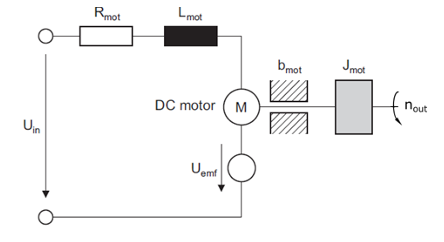
\includegraphics[width=0.45\textwidth]{img/Schematic representation of the electro-mechanical system.png}
  \caption[Schematic representation of the DC motor]{Schematic representation
    of the electro-mechanical system of the DC motor \cite{laboranleitung}}
  \label{fig:schematic}
\end{figure}

Kirchhoff's voltage law for the armature circuit with the back electromotive
force $u_\mathrm{emf} = k_\mathrm{E}\,\omega$ yields
Equation~\eqref{eq:electrical}, the balance of torques at the rotor yields
Equation~\eqref{eq:mechanical}.
\begin{equation}
  u(t) = R\,i(t) + L\,\frac{\mathrm{d}i(t)}{\mathrm{d}t} + k_\mathrm{E}\,\omega(t)
  \label{eq:electrical}
\end{equation}
\begin{equation}
  J\,\frac{\mathrm{d}\omega(t)}{\mathrm{d}t} = k_\mathrm{M}\,i(t) - b\,\omega(t)
  \label{eq:mechanical}
\end{equation}
\begin{legendtable}{@{}l@{\quad}l@{\qquad}l@{\quad}l@{}}
  $u$        & armature voltage, in \unit{\volt}
    & $J$            & rotor inertia, in \unit{\kilogram\metre\squared} \\
  $i$        & armature current, in \unit{\ampere}
    & $b$            & viscous friction, in \unit{\newton\metre\second\per\radian} \\
  $\omega$   & angular velocity, in \unit{\radian\per\second}
    & $k_\mathrm{M}$ & torque constant, in \unit{\newton\metre\per\ampere} \\
  $R$        & armature resistance, in \unit{\ohm}
    & $k_\mathrm{E}$ & back-EMF constant, in \unit{\volt\second\per\radian} \\
  $L$        & armature inductance, in \unit{\henry}
    & $t$            & time, in \unit{\second}
\end{legendtable}

\medskip\noindent
With $\omega = \mathrm{d}\theta/\mathrm{d}t$ for the angular position $\theta$,
the Laplace transformation (capital letters, Laplace variable $s$) yields the
transfer function from the voltage to the angular velocity, which is a
second-order lag element (PT2), and to the angular position, which additionally
contains an integrator. The derivation, both transfer functions and the
state-space model are given in Appendix~\ref{app:model}.

\section{System Identification}\label{sec:identification}
% Daten: matlab.mat (resp_12V), Fit: squarefit.m / PT2.m
The step response is recorded for an input step of $u_0 = \qty{12}{\volt}$ at
$t = \qty{0}{\second}$ with a sample time of
\qty{0.1}{\milli\second}~\cite{laboranleitung}. The encoder provides the
rotational speed $n$ of the output shaft in \unit{\per\minute} (resolution
\qty{1}{\per\minute}), which is converted into
$\omega = 2\pi n / \qty{60}{\second\per\minute}$; $\omega$ thus refers to the
output shaft, which is slower than the motor shaft by the factor $N$. The plant
is approximated by an overdamped PT2 element according to
Equation~\eqref{eq:pt2} with the static gain $K$ in
\unit{\radian\per\second\per\volt} and the time constants $\tau_1$, $\tau_2$ in
\unit{\second}.
\begin{equation}
  G_\mathrm{PT2}(s) = \frac{\Omega(s)}{U(s)}
  = \frac{K}{(\tau_1 s + 1)(\tau_2 s + 1)}
  \label{eq:pt2}
\end{equation}
$K$, $\tau_1$ and $\tau_2$ are determined by a least-squares fit of the step
response
\begin{equation*}
  \omega(t) = u_0 K \left[ 1 - \frac{\tau_1\,\mathrm{e}^{-t/\tau_1}
  - \tau_2\,\mathrm{e}^{-t/\tau_2}}{\tau_1 - \tau_2} \right]
\end{equation*}
to the measurement with the MATLAB function \texttt{lsqcurvefit}. Integrating
the angular velocity gives the plant for the position control in
Equation~\eqref{eq:pt3}~\cite{laboranleitung}.
\begin{equation}
  G_\mathrm{p}(s) = \frac{\Theta(s)}{U(s)} = \frac{1}{s}\,G_\mathrm{PT2}(s)
  = \frac{K}{s\,(\tau_1 s + 1)(\tau_2 s + 1)}
  \label{eq:pt3}
\end{equation}

\section{Controller Design and Implementation}\label{sec:design}
% Ziegler--Nichols Methode 2 (squarefit.m): rlocus -> K_cr, P_cr
A PID controller according to Equation~\eqref{eq:pid} with the proportional
gain $K_\mathrm{P}$ in \unit{\volt\per\radian}, the integral and derivative times
$T_\mathrm{I}$, $T_\mathrm{D}$ in \unit{\second}, $K_\mathrm{I} = K_\mathrm{P}/T_\mathrm{I}$
and $K_\mathrm{D} = K_\mathrm{P}\,T_\mathrm{D}$ is designed with the closed-loop
method of Ziegler and Nichols~\cite{ziegler1942}.
\begin{equation}
  G_\mathrm{c}(s) = K_\mathrm{P} \left( 1 + \frac{1}{T_\mathrm{I}\,s}
  + T_\mathrm{D}\,s \right)
  = K_\mathrm{P} + \frac{K_\mathrm{I}}{s} + K_\mathrm{D}\,s
  \label{eq:pid}
\end{equation}
The critical gain $K_\mathrm{cr}$, at which the closed loop of $G_\mathrm{p}(s)$
with a pure P controller reaches the stability limit, is determined from the
root locus with the MATLAB function \texttt{rlocus}, and the period
$P_\mathrm{cr}$ of the sustained oscillation from the simulated output
signal~\cite{laboranleitung}. The tuning rules $K_\mathrm{P} = 0.6\,K_\mathrm{cr}$,
$T_\mathrm{I} = 0.5\,P_\mathrm{cr}$ and $T_\mathrm{D} = 0.125\,P_\mathrm{cr}$
then give the controller parameters~\cite{ziegler1942}. The closed loop is
simulated in Simulink, with the reference converted from degrees into radians
before the controller and the output converted back~\cite{laboranleitung}.

\label{sec:implementation}
% Einstellungen aus RunPositionController1.slx, Parameter aus Controll_eng_pid_tuning.xlsx
The controller is implemented in Simulink Desktop Real-Time with a sample time
of \qty{0.1}{\milli\second}, in the parallel form of Equation~\eqref{eq:pid}
with a first-order derivative filter (coefficient \qty{100}{\per\second}). The
control value is limited to \qty{\pm 12}{\volt}, and integrator windup is
prevented by clamping. For each run, a reference step of \ang{45} is recorded
for \qty{1}{\second}, while $K_\mathrm{P}$, $K_\mathrm{I}$ and $K_\mathrm{D}$ are
varied one after another. In addition, a disturbance applied to the pointer and
the tracking of a sinusoidal reference are recorded.
